\documentclass[english]{article}
\usepackage{fullpage}
\usepackage{setspace}
\usepackage{color}
\usepackage{hyperref}

\usepackage[T1]{fontenc}
\usepackage[latin9]{inputenc}
\usepackage{amsthm}
\usepackage{amsmath}
\usepackage{amssymb}
\usepackage{graphicx}
\usepackage{dsfont}
\usepackage{cite}
\usepackage{amsmath}
\usepackage{array}
\usepackage{multirow}
\usepackage{caption}
\usepackage{color}


\usepackage{multicol}

\theoremstyle{plain}
\newtheorem{claim}{\protect\claimname}
\theoremstyle{plain}
\newtheorem{prop}{\protect\propositionname}
\theoremstyle{plain}
\newtheorem{lem}{\protect\lemmaname}
\theoremstyle{plain}
\newtheorem{thm}{\protect\theoremname}
\theoremstyle{plain}
\newtheorem{cor}{\protect\corollaryname}  
\theoremstyle{definition}
\newtheorem{defn}{\protect\definitionname}
\theoremstyle{definition}
\newtheorem{assump}{\protect\assumptionname}
\theoremstyle{definition}
\newtheorem{rem}{\protect\remarkname}

\makeatother
  
\usepackage{babel} 

\providecommand{\claimname}{Claim}
\providecommand{\lemmaname}{Lemma}
\providecommand{\propositionname}{Proposition}
\providecommand{\theoremname}{Theorem}
\providecommand{\corollaryname}{Corollary} 
\providecommand{\definitionname}{Definition}
\providecommand{\assumptionname}{Assumption}
\providecommand{\remarkname}{Remark}

\newcommand{\overbar}[1]{\mkern 1.25mu\overline{\mkern-1.25mu#1\mkern-0.25mu}\mkern 0.25mu}
\newcommand{\overbarr}[1]{\mkern 3.5mu\overline{\mkern-3.5mu#1\mkern-0.75mu}\mkern 0.75mu}
\newcommand{\mytilde}[1]{\mkern 0.5mu\widetilde{\mkern-0.5mu#1\mkern-0mu}\mkern 0mu}
\newcommand{\mytildee}[1]{\mkern 1.5mu\widetilde{\mkern-1.5mu#1\mkern-0mu}\mkern 0mu}
  
\DeclareMathOperator*{\argmax}{arg\,max}
\DeclareMathOperator*{\argmin}{arg\,min}
\DeclareMathOperator*{\maximize}{maximize}
\DeclareMathOperator*{\minimize}{minimize} 
\newcommand{\openone}{\mathds{1}}

\newcommand{\todo}{\bf \color{red} [TODO]~}

% Lecture notes
\newcommand{\Loss}{\mathrm{Loss}}
\newcommand{\wv}{\mathbf{w}}
\newcommand{\ptilde}{\widetilde{p}}
\newcommand{\bzeta}{\boldsymbol{\zeta}}
\newcommand{\bPhi}{\boldsymbol{\Phi}}
\newcommand{\Dtrain}{\mathcal{D}_{\mathrm{train}}}
\newcommand{\Dval}{\mathcal{D}_{\mathrm{val}}}
\newcommand{\Dtest}{\mathcal{D}_{\mathrm{test}}}
\newcommand{\Mc}{\mathcal{M}}
\newcommand{\mineq}{m_{\mathrm{ineq}}}
\newcommand{\meq}{m_{\mathrm{eq}}}
\newcommand{\ferm}{f_{\mathrm{erm}}}
\newcommand{\err}{\mathrm{err}}
\newcommand{\dVC}{d_{\mathrm{VC}}}
\newcommand{\Fall}{\mathcal{F}_{\mathrm{all}}}
\newcommand{\fopt}{f_{\mathrm{opt}}}
\newcommand{\BIC}{\mathrm{BIC}}
\newcommand{\AIC}{\mathrm{AIC}}
\newcommand{\bdelta}{\boldsymbol{\delta}}
\newcommand{\Rchat}{\widehat{\mathcal{R}}}

% Ranking and bandits
\newcommand{\thetamin}{\theta_{\mathrm{min}}}
\newcommand{\thetamax}{\theta_{\mathrm{max}}}
\newcommand{\Xhat}{\widehat{X}}
\newcommand{\Ghat}{\widehat{G}}
\newcommand{\jworst}{j_{\mathrm{worst}}}
\newcommand{\Actil}{\widetilde{\mathcal{A}}}
% \newcommand{\Stil}{\widetilde{S}}
\newcommand{\mab}{\texttt{mab}}
\newcommand{\cmp}{\texttt{cmp}}
\newcommand{\pemab}{P_{\mathrm{e},\texttt{mab}}}
\newcommand{\pecmp}{P_{\mathrm{e},\texttt{cmp}}}
\newcommand{\btheta}{\boldsymbol{\theta}}
\newcommand{\Alg}{\mathrm{ALG}}
\newcommand{\Geometric}{\mathrm{Geometric}}
\newcommand{\Ttotal}{T_{\mathrm{total}}}

% NoisyDD
\newcommand{\NDhat}{\widehat{\mathrm{ND}}}
\newcommand{\PDhat}{\widehat{\mathrm{PD}}}
% \newcommand{\Dhat}{\widehat{\mathrm{D}}}
\newcommand{\Shat}{\widehat{S}}
\newcommand{\peid}{P_{\mathrm{e},1}^{(\mathrm{D})}}
\newcommand{\peind}{P_{\mathrm{e},1}^{(\mathrm{ND})}}
\newcommand{\peiid}{P_{\mathrm{e},1}^{(\mathrm{D})}}
\newcommand{\peiind}{P_{\mathrm{e},1}^{(\mathrm{ND})}}
\newcommand{\epsid}{\epsilon_{1}^{(\mathrm{D})}}
\newcommand{\epsind}{\epsilon_{1}^{(\mathrm{ND})}}
\newcommand{\epsiid}{\epsilon_{2}^{(\mathrm{D})}}
\newcommand{\epsiind}{\epsilon_{2}^{(\mathrm{ND})}}
\newcommand{\nid}{n_1^{(\mathrm{D})}}
\newcommand{\nind}{n_1^{(\mathrm{ND})}}
\newcommand{\niid}{n_2^{(\mathrm{D})}}
\newcommand{\niind}{n_2^{(\mathrm{ND})}}
\newcommand{\Npd}{N_{\mathrm{pos}}^{(\mathrm{D})}}
\newcommand{\Npnd}{N_{\mathrm{pos}}^{(\mathrm{ND})}}
\newcommand{\npd}{n_{\mathrm{pos}}^{(\mathrm{D})}}
\newcommand{\npnd}{n_{\mathrm{pos}}^{(\mathrm{ND})}}
\newcommand{\npos}{n_{\mathrm{pos}}}
\newcommand{\nneg}{n_{\mathrm{neg}}}
\newcommand{\Ntilpos}{\widetilde{N}_{\mathrm{pos}}}
% \newcommand{\Npos}{N_{\mathrm{pos}}}
% \newcommand{\Nneg}{N_{\mathrm{neg}}}
\newcommand{\Aid}{\mathcal{A}_{1,i}^{(\mathrm{D})}}
\newcommand{\Aind}{\mathcal{A}_{1,i}^{(\mathrm{ND})}}
\newcommand{\mutild}{\tilde{\mu}^{(\mathrm{D})}}
\newcommand{\mutilnd}{\tilde{\mu}^{(\mathrm{ND})}}

% OneDimBO

\newcommand{\diag}{\mathrm{diag}}
\newcommand{\cunder}{\underline{c}}
\newcommand{\cbar}{\overline{c}}
\newcommand{\mutil}{\widetilde{\mu}}
\newcommand{\sigmatil}{\widetilde{\sigma}}
\newcommand{\Tearly}{T_{\mathrm{early}}}
\newcommand{\Tlate}{T_{\mathrm{late}}}
\newcommand{\Rearly}{R_{\mathrm{early}}}
\newcommand{\Rlate}{R_{\mathrm{late}}}
\newcommand{\Ctil}{\widetilde{C}}
\newcommand{\ctil}{\widetilde{c}}
\newcommand{\ftil}{\widetilde{f}}
\newcommand{\UCB}{\mathrm{UCB}}
\newcommand{\LCB}{\mathrm{LCB}}
\newcommand{\UCBtil}{\widetilde{\mathrm{UCB}}}
\newcommand{\LCBtil}{\widetilde{\mathrm{LCB}}}
\newcommand{\Lctil}{\widetilde{\mathcal{L}}}

% NoisyAdaptiveGT

\newcommand{\nMIi}{n_{\mathrm{MI,1}}}
\newcommand{\nMIii}{n_{\mathrm{MI,2}}}
\newcommand{\nConc}{n_{\mathrm{Conc}}}
\newcommand{\nIndiv}{n_{\mathrm{Indiv}}}
\newcommand{\nHalving}{n_{\mathrm{Halving}}}
\newcommand{\kmax}{k_{\mathrm{max}}}
\newcommand{\ptil}{\widetilde{p}}
\newcommand{\elltil}{\widetilde{\ell}}
\newcommand{\Stil}{\widetilde{S}}
\newcommand{\ncheck}{\check{n}}

% SeparateGT

\newcommand{\cmean}{c_{\mathrm{mean}}}
\newcommand{\cvar}{c_{\mathrm{var}}}
\newcommand{\ccov}{c_{\mathrm{cov}}}
\newcommand{\cmax}{c_{\mathrm{max}}}

\newcommand{\dneg}{d_{\mathrm{neg}}}
\newcommand{\dpos}{d_{\mathrm{pos}}}
\newcommand{\Nneg}{N_{\mathrm{neg}}}
\newcommand{\Npos}{N_{\mathrm{pos}}}
\newcommand{\Nerr}{N_{\mathrm{err}}}
\newcommand{\alphaneg}{\alpha_{\mathrm{neg}}}
\newcommand{\alphapos}{\alpha_{\mathrm{pos}}}

\newcommand{\pej}{P_{\mathrm{e},j}}
\newcommand{\nusymm}{\nu_{\mathrm{symm}}}

% PooledData
\newcommand{\bpi}{\boldsymbol{\pi}}
\newcommand{\Nrm}{\mathrm{N}}
\newcommand{\CNrm}{\mathrm{CN}}

% ConverseGP
\newcommand{\vbar}{\overline{v}}

% GT_ICASSP

\newcommand{\pc}{P_{\mathrm{c}}}

% ActiveMRF

\newcommand{\lammin}{\lambda_{\mathrm{min}}}
\newcommand{\lammax}{\lambda_{\mathrm{max}}}
\newcommand{\missing}{\ast}
\newcommand{\pFAi}{p_{\mathrm{FA},i}}
\newcommand{\pMDi}{p_{\mathrm{MD},i}}
\newcommand{\bSigmatil}{\widetilde{\mathbf{\Sigma}}}
\newcommand{\mtil}{\widetilde{m}}
\newcommand{\Ptil}{\widetilde{P}}
\newcommand{\dmin}{d_{\mathrm{min}}}
\newcommand{\davg}{d_{\mathrm{avg}}}
\newcommand{\dmaxbar}{\overline{d}_{\mathrm{max}}}
\newcommand{\taumin}{\tau_{\mathrm{min}}}
\newcommand{\taumax}{\tau_{\mathrm{max}}}
\newcommand{\ntil}{\widetilde{n}}
\newcommand{\Ntil}{\widetilde{N}}
\newcommand{\Ncheck}{\check{N}}
\newcommand{\kbar}{\overbar{k}}

\newcommand{\mmin}{m_{\mathrm{min}}}
\newcommand{\mmax}{m_{\mathrm{max}}}

% PartialSBM
\newcommand{\ellv}{\boldsymbol{\ell}}
\newcommand{\Cieq}{C_{1,\mathrm{eq}}}
\newcommand{\Cidif}{C_{1,\mathrm{dif}}}
\newcommand{\Ctilde}{\tilde{C}}
\newcommand{\dbar}{\overline{d}}
\newcommand{\bsigma}{\boldsymbol{\sigma}}
\newcommand{\Poisson}{\mathrm{Poisson}}
\newcommand{\ktilde}{\tilde{k}}
 
% GT_ISIT
\newcommand{\Veq}{V_{\mathrm{eq}}}
\newcommand{\Vdif}{V_{\mathrm{dif}}}
\newcommand{\Vveq}{\mathbf{V}_{\mathrm{eq}}}
\newcommand{\Vvdif}{\mathbf{V}_{\mathrm{dif}}}
\newcommand{\veq}{v_{\mathrm{eq}}}
\newcommand{\vdif}{v_{\mathrm{dif}}}

%
% MultiMRI
%
\newcommand{\bpsi}{\boldsymbol{\psi}}

%
% Group testing 
%
\newcommand{\Hg}{\mathrm{Hypergeometric}}
\newcommand{\TV}{\mathrm{TV}}
\newcommand{\dTV}{d_{\mathrm{TV}}}

%
% Graphical model selection
%
\newcommand{\Gbar}{\overbar{G}}
\newcommand{\Mbar}{\overbar{M}}
\newcommand{\qmax}{q_{\mathrm{max}}}

%
% Community detection
%
\newcommand{\Bi}{\mathrm{Binomial}}
\newcommand{\Hc}{\mathcal{H}}
\newcommand{\Ev}{\mathbf{E}}

%
% Support recovery
%
\newcommand{\Sbar}{\overbar{S}}
\newcommand{\sbar}{\overbar{s}}

%\newcommand{\Wdif}{W_{\mathrm{dif}}}
%\newcommand{\Weq}{W_{\mathrm{eq}}}
%\newcommand{\wdif}{w_{\mathrm{dif}}}
%\newcommand{\weq}{w_{\mathrm{eq}}}

\newcommand{\Sdif}{S_{\mathrm{dif}}}
\newcommand{\Seq}{S_{\mathrm{eq}}}
\newcommand{\sdif}{s_{\mathrm{dif}}}
\newcommand{\sdifbar}{\overbar{s}_{\mathrm{dif}}}
\newcommand{\seqbar}{\overbar{s}_{\mathrm{eq}}}
\newcommand{\seq}{s_{\mathrm{eq}}}
\newcommand{\sdifhat}{\hat{s}_{\mathrm{dif}}}
\newcommand{\sdifx}{\overbar{s} \backslash s}
\newcommand{\seqx}{\overbar{s} \cap s}

\newcommand{\Xvdif}{\mathbf{X}_{\overbar{s} \backslash s}}
\newcommand{\Xveq}{\mathbf{X}_{\overbar{s} \cap s}}
\newcommand{\Xvdifo}{\mathbf{X}_{s \backslash \overbar{s}}}
\newcommand{\xvdif}{\mathbf{x}_{\overbar{s} \backslash s}}
\newcommand{\xveq}{\mathbf{x}_{\overbar{s} \cap s}}
\newcommand{\xveqo}{\mathbf{x}_{s \backslash \overbar{s}}}

\newcommand{\Ord}{\mathcal{O}}
\newcommand{\Yctil}{\widetilde{\mathcal{Y}}}

\newcommand{\dmax}{d_{\mathrm{max}}}
\newcommand{\dH}{d_{\mathrm{H}}}

\newcommand{\jeq}{j_{\mathrm{eq}}}
\newcommand{\jdiff}{j_{\mathrm{dif}}}

\newcommand{\Zhat}{\hat{Z}}
\newcommand{\Zhatmax}{\hat{Z}_{\mathrm{max}}}
\newcommand{\zdiff}{z_{\mathrm{dif}}}
\newcommand{\zcomm}{z_{\mathrm{eq}}}

\newcommand{\bmin}{b_{\mathrm{min}}}
\newcommand{\Bmin}{\beta_{\mathrm{min}}}
\newcommand{\bmax}{b_{\mathrm{max}}}
\newcommand{\sigbeta}{\sigma_{\beta}}
\newcommand{\siglv}{\sigma_{\sdif}}
\newcommand{\Tr}{\mathrm{Tr}}

\newcommand{\sign}{\mathrm{sign}}
\newcommand{\SNRdB}{\mathrm{SNR}_{\mathrm{dB}}}

\newcommand{\Weq}{W_{\mathrm{eq}}}
\newcommand{\Wdif}{W_{\mathrm{dif}}}
\newcommand{\weq}{w_{\mathrm{eq}}}
\newcommand{\wdif}{w_{\mathrm{dif}}}
\newcommand{\feq}{f_{\mathrm{eq}}}
\newcommand{\fdif}{f_{\mathrm{dif}}}

\newcommand{\bgood}{b_{\mathrm{good}}}
\newcommand{\bbad}{b_{\mathrm{bad}}}

\newcommand{\btil}{\widetilde{b}}
\newcommand{\betatil}{\widetilde{\beta}}
\newcommand{\betatileq}{\widetilde{\beta}_{\mathrm{eq}}}
\newcommand{\betatildif}{\widetilde{\beta}_{\mathrm{dif}}}
\newcommand{\btileq}{\widetilde{b}_{\mathrm{eq}}}
\newcommand{\btildif}{\widetilde{b}_{\mathrm{dif}}}
\newcommand{\stileq}{\widetilde{s}_{\mathrm{eq}}}
\newcommand{\stildif}{\widetilde{s}_{\mathrm{dif}}}
\newcommand{\pieq}{\pi_{\mathrm{eq}}}
\newcommand{\pidif}{\pi_{\mathrm{dif}}}
\newcommand{\Sdifhat}{\hat{S}_{\mathrm{dif}}}

\newcommand{\Bcfano}{\mathcal{B}'_{\mathrm{Fano}}}

\newcommand{\Sceq}{\mathcal{S}_{\mathrm{eq}}}
\newcommand{\Scdif}{\mathcal{S}_{\mathrm{dif}}}
\newcommand{\Nc}{\mathcal{N}}

%
% From MultiMRI
%
\newcommand{\Pv}{\mathbf{P}}
\newcommand{\Wvtil}{\widetilde{\mathbf{W}}}
\newcommand{\wtil}{\widetilde{w}}
\newcommand{\xvhat}{\hat{\mathbf{x}}}

%
% From Expanders_FOCS
%
\newcommand{\Bernoulli}{\mathrm{Bernoulli}}
\newcommand{\Binomial}{\mathrm{Binomial}}
\newcommand{\imtil}{\tilde{\imath}}
\newcommand{\SNR}{\mathrm{SNR}}

%
% From PaperBI
%
\newcommand{\CLM}{C_{\mathrm{LM}}}
\newcommand{\CSC}{C_{\mathrm{SC}}}
\newcommand{\ISC}{I_{\mathrm{SC}}}
\newcommand{\CM}{C_{\mathrm{M}}}
\newcommand{\Qmin}{Q_{\mathrm{min}}}
\newcommand{\Phat}{\widehat{P}}

%
% From JournalSU
%
\newcommand{\pebar}{\overbar{P}_{\mathrm{e}}}
\newcommand{\petilde}{\tilde{p}_{\mathrm{e}}}
\newcommand{\pe}{P_{\mathrm{e}}}
\newcommand{\pen}{P_{\mathrm{e},n}}
\newcommand{\peQ}{P_{\mathrm{e},Q}} 
\newcommand{\pemax}{P_{\mathrm{e},\mathrm{max}}} 
\newcommand{\msg}{\mathsf{m}}

\newcommand{\Ez}{E_{0}}
\newcommand{\Er}{E_{\mathrm{r}}}
\newcommand{\Esp}{E_{\mathrm{sp}}}
\newcommand{\Eziid}{E_{0}^{\mathrm{iid}}}
\newcommand{\Ezcc}{E_{0}^{\mathrm{cc}}}
\newcommand{\Eohatcc}{\hat{E}_{0}^{\mathrm{cc}}}
\newcommand{\Eohatcost}{\hat{E}_{0}^{\mathrm{cost}}}
\newcommand{\Ezcost}{E_{0}^{\mathrm{cost}}}
\newcommand{\Ezcostprime}{E_{0}^{\mathrm{cost}^{\prime}}}
\newcommand{\Eriid}{E_{\mathrm{r}}^{\mathrm{iid}}}
\newcommand{\Ercc}{E_{\mathrm{r}}^{\mathrm{cc}}}
\newcommand{\Erccprime}{E_{\mathrm{r},12}^{\mathrm{cc}^{\prime}}}
\newcommand{\Ercost}{E_{\mathrm{r}}^{\mathrm{cost}}}
\newcommand{\Ercostprime}{E_{\mathrm{r}}^{\mathrm{cost}^{\prime}}}

\newcommand{\rcu}{\mathrm{rcu}}
\newcommand{\rcus}{\rcu_{s}}
\newcommand{\rcuss}{\rcu_{s}^{*}}
\newcommand{\rcusa}{\rcu_{s,a}^{*}}
\newcommand{\rcushat}{\widehat{\mathrm{rcu}}_{s}}
\newcommand{\rcusshat}{\widehat{\mathrm{rcu}}_{s}^{*}}
\newcommand{\alphasa}{\alpha^{\mathrm{iid}}}
\newcommand{\rcul}{\rcu_{\mathrm{L}}}
\newcommand{\rhohat}{\hat{\rho}}
\newcommand{\LM}{I_{\mathrm{LM}}}
\newcommand{\GMI}{I_{\mathrm{GMI}}}

\newcommand{\SetScc}{\mathcal{S}}
\newcommand{\SetSncc}{\mathcal{S}_{n}}
\newcommand{\SetSncost}{\mathcal{S}_{n}}
\newcommand{\SetSiid}{\mathcal{S}^{\mathrm{iid}}}
\newcommand{\SetScost}{\mathcal{S}}
\newcommand{\SetSniid}{\mathcal{S}_{n}^{\mathrm{iid}}}
\newcommand{\SetTcc}{\mathcal{T}}
\newcommand{\SetTiid}{\mathcal{T}^{\mathrm{iid}}}
\newcommand{\SetTcost}{\mathcal{T}}
\newcommand{\SetTncost}{\mathcal{T}_{n}}
\newcommand{\SetTncc}{\mathcal{T}_{n}}

\newcommand{\Miid}{M^{\mathrm{iid}}}
\newcommand{\Mcc}{M^{\mathrm{cc}}}
\newcommand{\Mcost}{M^{\mathrm{cost}}}
\newcommand{\Rcr}{R_{\mathrm{cr}}}
\newcommand{\Rcrs}{R_s^{\mathrm{cr}}}

\newcommand{\Fbar}{\overbar{F}}
\newcommand{\Funder}{\underline{F}}
\newcommand{\Gunder}{\underline{G}}
\newcommand{\PXv}{P_{\Xv}}
\newcommand{\qbar}{\overbar{q}}
\newcommand{\rbar}{\overbar{r}}
\newcommand{\rtilde}{\tilde{r}}
\newcommand{\atilde}{\tilde{a}}
\newcommand{\phitilde}{\tilde{\phi}}
\newcommand{\Mtilde}{\mytildee{M}}
\newcommand{\Ptilde}{\widetilde{P}}
\newcommand{\Qtilde}{\widetilde{Q}}
\newcommand{\Etilde}{\widetilde{E}}
\newcommand{\Rtilde}{\mytildee{R}}
\newcommand{\Wtilde}{\widetilde{W}}
\newcommand{\Wvtilde}{\widetilde{\mathbf{W}}}
\newcommand{\hover}{\overbar{h}}
\newcommand{\ubar}{\overbar{u}}
\newcommand{\Ubar}{\overbar{U}}
\newcommand{\xbarbar}{\overbar{\overbar{x}}}
\newcommand{\Xbarbar}{\overbar{\overbar{X}}}
\newcommand{\xbar}{\overbar{x}}
\newcommand{\Xbar}{\overbar{X}}
\newcommand{\xtilde}{\widetilde{x}}
\newcommand{\Xtilde}{\mytilde{X}}
\newcommand{\ybar}{\overbar{y}}
\newcommand{\zbar}{\overbar{z}}
\newcommand{\Zbar}{\overbar{Z}}
\newcommand{\thetabar}{\overbar{\theta}}

\newcommand{\av}{\mathbf{a}}
\newcommand{\Qv}{\mathbf{Q}}
\newcommand{\uvbar}{\overbar{\mathbf{u}}}
\newcommand{\uv}{\mathbf{u}}
\newcommand{\Uvbar}{\overbar{\mathbf{U}}}
\newcommand{\Uv}{\mathbf{U}}
\newcommand{\vv}{\mathbf{v}}
\newcommand{\Vv}{\mathbf{V}}
\newcommand{\vvbar}{\overbar{\mathbf{v}}}
\newcommand{\xvbarbar}{\overbar{\overbar{\mathbf{x}}}}
\newcommand{\xvbar}{\overbar{\mathbf{x}}}
\newcommand{\xvtilde}{\widetilde{\mathbf{x}}}
\newcommand{\xv}{\mathbf{x}}
\newcommand{\Xvbarbar}{\overbar{\overbar{\mathbf{X}}}}
\newcommand{\Xvbar}{\overbar{\mathbf{X}}}
\newcommand{\Xvtilde}{\mytilde{\mathbf{X}}}
\newcommand{\Ytilde}{\widetilde{Y}}
\newcommand{\Yvtilde}{\widetilde{\mathbf{Y}}}
\newcommand{\Xv}{\mathbf{X}}
\newcommand{\yv}{\mathbf{y}}
\newcommand{\Yv}{\mathbf{Y}}
\newcommand{\zv}{\mathbf{z}}
\newcommand{\Zv}{\mathbf{Z}}

\newcommand{\Yvs}{\mathbf{Y}_{\hspace*{-0.5ex}s}}
\newcommand{\Uvn}{\mathbf{U}_{\hspace*{-0.3ex}n}}
\newcommand{\Tvn}{\mathbf{T}_{\hspace*{-0.3ex}n}} 
\newcommand{\Vvi}{\mathbf{V}_{\hspace*{-0.3ex}1}} 
\newcommand{\Vvii}{\mathbf{V}_{\hspace*{-0.3ex}2}}
\newcommand{\Vvm}{\mathbf{V}_{\hspace*{-0.3ex}m}}
\newcommand{\Vvtilden}{\widetilde{\mathbf{V}}_{\hspace*{-0.3ex}n}}   
\newcommand{\QUn}{Q_{U\hspace*{-0.2ex},\hspace*{0.05ex}n}}
\newcommand{\QXgUn}{Q_{X|U\hspace*{-0.2ex},\hspace*{0.05ex}n}}
\newcommand{\QUXn}{Q_{UX\hspace*{-0.2ex},\hspace*{0.05ex}n}}
\newcommand{\Yvi}{\mathbf{Y}_{\hspace*{-0.5ex}1}}
\newcommand{\Yvii}{\mathbf{Y}_{\hspace*{-0.5ex}2}}
\newcommand{\Yvu}{\mathbf{Y}_{\hspace*{-0.5ex}u}}

\newcommand{\Ac}{\mathcal{A}}
\newcommand{\Bc}{\mathcal{B}}
\newcommand{\Cc}{\mathcal{C}}
\newcommand{\Dc}{\mathcal{D}}
\newcommand{\Ec}{\mathcal{E}}
\newcommand{\Fc}{\mathcal{F}}
\newcommand{\Gc}{\mathcal{G}}
\newcommand{\ic}{\mathcal{i}}
\newcommand{\Ic}{\mathcal{I}}
\newcommand{\Kc}{\mathcal{K}}
\newcommand{\Pc}{\mathcal{P}}
\newcommand{\Sc}{\mathcal{S}}
\newcommand{\Tc}{\mathcal{T}}
\newcommand{\Uc}{\mathcal{U}}
\newcommand{\Wc}{\mathcal{W}}
\newcommand{\Xc}{\mathcal{X}}
\newcommand{\Yc}{\mathcal{Y}}
\newcommand{\Zc}{\mathcal{Z}}

\newcommand{\CC}{\mathbb{C}}
\newcommand{\EE}{\mathbb{E}}
\newcommand{\PP}{\mathbb{P}}
\newcommand{\RR}{\mathbb{R}}
\newcommand{\ZZ}{\mathbb{Z}}
\newcommand{\Qsf}{\mathsf{Q}}

\newcommand{\al}{\{a_l\}}
\newcommand{\rl}{\{r_l\}}
\newcommand{\rbarl}{\{\overbar{r}_l\}}
\newcommand{\defeq}{\triangleq}
\newcommand{\deq}{\stackrel{d}{=}}
\newcommand{\var}{\mathrm{Var}}
\newcommand{\cov}{\mathrm{Cov}}
\newcommand{\erfcxi}{\mathrm{erfcx}_{1}}
\newcommand{\erfcx}{\mathrm{erfcx}}
\newcommand{\erfc}{\mathrm{erfc}}
\newcommand{\supp}{\mathrm{supp}}

\newcommand{\alphanl}{\alpha^{\mathrm{nl}}_n}
\newcommand{\alphal}{\alpha^{\mathrm{l}}_n}
\newcommand{\betanl}{\beta^{\mathrm{nl}}_n}
\newcommand{\betal}{\beta^{\mathrm{l}}_n}

\newcommand{\Es}{E_{\mathrm{s}}}
\newcommand{\EJ}{E_{\mathrm{J}}}
\newcommand{\EJi}{E_{\mathrm{J},1}}
\newcommand{\EJii}{E_{\mathrm{J},2}}

\newcommand{\Vmin}{V_{\mathrm{min}}}
\newcommand{\Vmax}{V_{\mathrm{max}}}

%
% From PaperExpurgated
%

\newcommand{\rcux}{\mathrm{rcux}}

\newcommand{\Eexiid}{E_{\mathrm{ex}}^{\mathrm{iid}}}
\newcommand{\Eexcc}{E_{\mathrm{ex}}^{\mathrm{cc}}}
\newcommand{\Eexhatcc}{\hat{E}_{\mathrm{ex}}^{\mathrm{cc}}}
\newcommand{\Eexcost}{E_{\mathrm{ex}}^{\mathrm{cost}}}
\newcommand{\Eexcostprime}{E_{\mathrm{ex}}^{\mathrm{cost}^{\prime}}}
\newcommand{\Exiid}{E_{\mathrm{x}}^{\mathrm{iid}}}
\newcommand{\Excc}{E_{\mathrm{x}}^{\mathrm{cc}}}
\newcommand{\Excost}{E_{\mathrm{x}}^{\mathrm{cost}}}
\newcommand{\Excoststar}{E_{\mathrm{x}}^{\mathrm{cost}^{*}}}
\newcommand{\Excostprime}{E_{\mathrm{x}}^{\mathrm{cost}^{\prime}}}
\newcommand{\Eex}{E_{\mathrm{ex}}}
\newcommand{\Ex}{E_{\mathrm{x}}}

\newcommand{\Pxbicm}{P_{X}^{\rm bicm}}

\newcommand{\Av}{\mathbf{A}}
\newcommand{\Bv}{\mathbf{B}}
\newcommand{\bv}{\mathbf{b}}
\newcommand{\mbar}{\overbar{m}}
\newcommand{\tv}{\mathbf{t}}

\newcommand{\Lsf}{\mathsf{L}}
\newcommand{\Csf}{\mathsf{C}}
\newcommand{\csf}{\mathsf{c}}
\newcommand{\Fsf}{\mathsf{F}}
\newcommand{\Tsf}{\mathsf{T}}

\newcommand{\brl}{\{\overbar{r}_l\}}

%
% From DocumentMU
%

\newcommand{\peobar}{\overbar{p}_{\mathrm{e},0}}
\newcommand{\peibar}{\overbar{p}_{\mathrm{e},1}}
\newcommand{\peiibar}{\overbar{p}_{\mathrm{e},2}}
\newcommand{\peiiibar}{\overbar{p}_{\mathrm{e},12}}
\newcommand{\peo}{P_{\mathrm{e},0}}
\newcommand{\pei}{P_{\mathrm{e},1}}
\newcommand{\peii}{P_{\mathrm{e},2}}
\newcommand{\peiii}{P_{\mathrm{e},12}}
\newcommand{\rcuo}{\mathrm{rcu}_{0}}
\newcommand{\rcui}{\mathrm{rcu}_{1}}
\newcommand{\rcuii}{\mathrm{rcu}_{2}}
\newcommand{\rcuiii}{\mathrm{rcu}_{12}}
\newcommand{\rcuiiiprime}{\mathrm{rcu}_{12}^{\prime}}
\newcommand{\rcuiiia}{\mathrm{rcu}_{12,1}}
\newcommand{\rcuiiib}{\mathrm{rcu}_{12,2}}

\newcommand{\Eiziid}{E_{0,1}^{\mathrm{iid}}}
\newcommand{\Eiiziid}{E_{0,2}^{\mathrm{iid}}}
\newcommand{\Eiiiziid}{E_{0,12}^{\mathrm{iid}}}
\newcommand{\Eiiiaziid}{E_{0,12,1}^{\mathrm{iid}}}
\newcommand{\Eiiibziid}{E_{0,12,2}^{\mathrm{iid}}}
\newcommand{\Eozcc}{E_{0,0}^{\mathrm{cc}}}
\newcommand{\Eizcc}{E_{0,1}^{\mathrm{cc}}}
\newcommand{\Eiizcc}{E_{0,2}^{\mathrm{cc}}}
\newcommand{\Eiiizcc}{E_{0,12}^{\mathrm{cc}}}
\newcommand{\Eiiizccprime}{E_{0,12}^{\mathrm{cc}^{\prime}}}
\newcommand{\Eiiizccpprime}{E_{0,12}^{\mathrm{cc}^{\prime\prime}}}
\newcommand{\Eiiiazcc}{E_{0,12,1}^{\mathrm{cc}}}
\newcommand{\Eiiibzcc}{E_{0,12,2}^{\mathrm{cc}}}
\newcommand{\Ehatiiiazcc}{\hat{E}_{0,12,1}^{\mathrm{cc}}}
\newcommand{\Eozcost}{E_{0,0}^{\mathrm{cost}}}
\newcommand{\Eizcost}{E_{0,1}^{\mathrm{cost}}}
\newcommand{\Eiizcost}{E_{0,2}^{\mathrm{cost}}}
\newcommand{\Eiiizcost}{E_{0,12}^{\mathrm{cost}}}
\newcommand{\Eiiiazcost}{E_{0,12,1}^{\mathrm{cost}}}
\newcommand{\Eiiibzcost}{E_{0,12,2}^{\mathrm{cost}}}
\newcommand{\Eiiizaccts}{E_{0,12,1}^{\text{cc-ts}}}

\newcommand{\Eiriid}{E_{\mathrm{r},1}^{\mathrm{iid}}}
\newcommand{\Eiiriid}{E_{\mathrm{r},2}^{\mathrm{iid}}}
\newcommand{\Eiiiriid}{E_{\mathrm{r},12}^{\mathrm{iid}}}
\newcommand{\Eiiiariid}{E_{\mathrm{r},12,1}^{\mathrm{iid}}}
\newcommand{\Eiiibriid}{E_{\mathrm{r},12,2}^{\mathrm{iid}}}
\newcommand{\Eorcc}{E_{\mathrm{r},0}^{\mathrm{cc}}}
\newcommand{\Eorccprime}{E_{\mathrm{r},0}^{\mathrm{cc}^{\prime}}}
\newcommand{\Eircc}{E_{\mathrm{r},1}^{\mathrm{cc}}}
\newcommand{\Eiircc}{E_{\mathrm{r},2}^{\mathrm{cc}}}
\newcommand{\Eiiircc}{E_{\mathrm{r},12}^{\mathrm{cc}}}
\newcommand{\Eiiiarcc}{E_{\mathrm{r},12,1}^{\mathrm{cc}}}
\newcommand{\Eiiibrcc}{E_{\mathrm{r},12,2}^{\mathrm{cc}}}
\newcommand{\Eorcost}{E_{\mathrm{r},0}^{\mathrm{cost}}}
\newcommand{\Eircost}{E_{\mathrm{r},1}^{\mathrm{cost}}}
\newcommand{\Eiircost}{E_{\mathrm{r},2}^{\mathrm{cost}}}
\newcommand{\Eiiircost}{E_{\mathrm{r},12}^{\mathrm{cost}}}
\newcommand{\Eiiiarcost}{E_{\mathrm{r},12,1}^{\mathrm{cost}}}
\newcommand{\Eiiibrcost}{E_{\mathrm{r},12,2}^{\mathrm{cost}}}
\newcommand{\Eiiirtilde}{\widetilde{E}_{\mathrm{r,12}}}
\newcommand{\Eiiirccts}{E_{\mathrm{r},12}^{\text{cc-ts}}}

\newcommand{\Wsu}{W^{\prime}}
\newcommand{\qsu}{q^{\prime}}
\newcommand{\RegLM}{\mathcal{R}_{\mathrm{LM}}}
\newcommand{\RegLMex}{\mathcal{R}_{\mathrm{ex}}}

\newcommand{\SetSccts}{\mathcal{S}^{\mathrm{ts}}}
\newcommand{\SetTocc}{\mathcal{T}_0}
\newcommand{\SetToncc}{\mathcal{T}_{0,n}}
\newcommand{\SetTicc}{\mathcal{T}_{1}}
\newcommand{\SetTiicc}{\mathcal{T}_{2}}
\newcommand{\SetTiiicc}{\mathcal{T}_{12}}
\newcommand{\SetTiiincc}{\mathcal{T}_{12,n}}
\newcommand{\SetTnucc}{\mathcal{T}_{\nu}}
\newcommand{\SetTnuccex}{\mathcal{T}_{\nu}^{\mathrm{ex}}}
\newcommand{\SetTiccex}{\mathcal{T}_{1}^{\mathrm{ex}}}
\newcommand{\SetTiiccex}{\mathcal{T}_{2}^{\mathrm{ex}}}
\newcommand{\SetTiiiccex}{\mathcal{T}_{12}^{\mathrm{ex}}}
\newcommand{\SetTiccts}{\mathcal{T}_{1}^{\mathrm{ts}}}
\newcommand{\SetTiiccts}{\mathcal{T}_{2}^{\mathrm{ts}}}
\newcommand{\SetTiiiccts}{\mathcal{T}_{12}^{\mathrm{ts}}}

\newcommand{\qv}{\mathbf{q}}
\newcommand{\Wv}{\mathbf{W}}
\newcommand{\Rc}{\mathcal{R}}
\newcommand{\Vc}{\mathcal{V}}

\newcommand{\Rsc}{R^{\mathrm{sc}}}
\newcommand{\Rmac}{R^{\mathrm{ex}}}
\newcommand{\Rosc}{R_{0}^{\mathrm{sc}}}
\newcommand{\Risc}{R_{1}^{\mathrm{sc}}}
\newcommand{\Rimac}{R_{1}^{\mathrm{ex}}}
\newcommand{\Riimac}{R_{2}^{\mathrm{ex}}}
\newcommand{\Usc}{U^{\mathrm{sc}}}
\newcommand{\Ucsc}{\mathcal{U}^{\mathrm{sc}}}
\newcommand{\Ximac}{X_{1}^{\mathrm{ex}}}
\newcommand{\Xcimac}{\mathcal{X}_{1}^{\mathrm{ex}}}
\newcommand{\Xiimac}{X_{2}^{\mathrm{ex}}}
\newcommand{\Xciimac}{\mathcal{X}_{2}^{\mathrm{ex}}}

\newcommand{\PrML}{\PP^{(\mathrm{ML})}}
\newcommand{\PrS}{\PP^{(\mathrm{S})}}
\newcommand{\PrGenie}{\PP^{(\mathrm{Genie})}}

%
% From MAC2OR
%
\newcommand{\Lc}{\mathcal{L}}
\newcommand{\cv}{\mathbf{c}}
\newcommand{\Dv}{\mathbf{D}}
\newcommand{\Iv}{\mathbf{I}}
\newcommand{\iv}{\mathbf{i}}
\newcommand{\Fv}{\mathbf{F}}
\newcommand{\fv}{\mathbf{f}}
\newcommand{\Mv}{\mathbf{M}}
\newcommand{\Jv}{\mathbf{J}}
\newcommand{\Kv}{\mathbf{K}}
\newcommand{\kv}{\mathbf{k}}
\newcommand{\Lv}{\mathbf{L}}
\newcommand{\Rv}{\mathbf{R}}
\newcommand{\sv}{\mathbf{s}}
\newcommand{\Sv}{\mathbf{S}}
\newcommand{\Tv}{\mathbf{T}}
\newcommand{\bzero}{\boldsymbol{0}}
\newcommand{\bone}{\boldsymbol{1}}
\newcommand{\bmu}{\boldsymbol{\mu}}
\newcommand{\bnu}{\boldsymbol{\nu}}
\newcommand{\blambda}{\boldsymbol{\lambda}}
\newcommand{\balpha}{\boldsymbol{\alpha}}
\newcommand{\bphi}{\boldsymbol{\phi}}
\newcommand{\bgamma}{\boldsymbol{\gamma}}
\newcommand{\bTheta}{\boldsymbol{\Theta}}
\newcommand{\bOmega}{\boldsymbol{\Omega}}
\newcommand{\bSigma}{\boldsymbol{\Sigma}}
\newcommand{\bLambda}{\boldsymbol{\Lambda}}
\newcommand{\bPsi}{\boldsymbol{\Psi}}
\newcommand{\bDelta}{\boldsymbol{\Delta}}
\newcommand{\bell}{\boldsymbol{\ell}}
\newcommand{\Qinv}{\mathsf{Q}_{\mathrm{inv}}}

%
% From RefinementCC
%
\newcommand{\Wocc}{\mathcal{W}_{0}^{\mathrm{cc}}}
\newcommand{\Wosymm}{\mathcal{W}_{0}^{\mathrm{symm}}}
\newcommand{\Wsymm}{\mathcal{W}^{\mathrm{symm}}}
\newcommand{\Qocc}{\mathcal{Q}_{0}^{\mathrm{cc}}}
\newcommand{\Qc}{\mathcal{Q}}
\newcommand{\bxi}{\mathbf{\xi}}
\newcommand{\Ezxcc}{E_{0,x}^{\mathrm{cc}}}
\newcommand{\Ezxicc}{E_{0,x_{i}}^{\mathrm{cc}}}
\newcommand{\Rcrsa}{R_{s,a}^{\mathrm{cr}}}

\title{CS5339 Sample Project -- AdaBoost Algorithm}
\date{}
\author{Jonathan Scarlett}

\newcommand{\ntrain}{n_{\rm train}}
\newcommand{\ntest}{n_{\rm test}}

\onehalfspacing

\begin{document}
\maketitle

{\color{red} 
\section*{Notes on this Sample Project}

\begin{itemize}
    \item This project is only meant to give an example indication of style, format, etc., rather than being a model for an ``ideal'' project.   (Though, hypothetically, it could be considered one that would receive a fairly high grade)
    \item To avoid overlap with the suggested topics, this sample project is based on a topic that will be covered in the lectures.  Your own project should of course avoid significant overlap with the lectures (though comparisons/connections to that material can be highlighted).
    \item It is not necessary to include everything here (e.g., experiments, detailed proofs, extensions, citations to several published papers) in your report.  You should try to judge this based on your chosen topic and the assessment criteria.
    \item You may notice the use of the first-person ``we'' despite only having a single author.  This has become conventional in academic writing, but you can use the first-person ``I'' or the passive voice if you prefer.
    \item This sample report is relatively light on the ``Additional Material'' part regarding experiments and published papers, though it includes a bit of both.  You should ideally include slightly more in your own report.
\end{itemize}
}

\section{Introduction} \label{sec:intro}

The fundamental problem of binary classification is central to both classical and modern machine learning.  Many of the earliest works focused on simple classification rules, such as linear classifiers or nearest-neighbor rules, whereas more recent developments have led to more sophisticated ideas such as kernel methods, artificial neural networks, and more.  Many such methods can be viewed as {\em combining simple classifiers} to produce a {\em complex classifier}.

In this report, we will overview a famous algorithm falling under this category, known as AdaBoost, which was introduced by Freund and Schapire in 1997 \cite{freund1997decision}, and subsequently significantly impacted both the theory and practice of machine learning.  The authors were awarded the 2003 G\"odel prize, and the algorithm is often considered to be one one of the most effective ``off-the-shelf'' algorithms requiring minimal tuning and tweaking \cite{blog,wiki}.

Before proceeding with a formal description, we outline some of the main high-level concepts and ideas behind AdaBoost:
\begin{itemize}
    \item The algorithm is given a class of {\em weak learners}, also known as {\em base learners}, containing classifiers that are not very powerful in themselves.  Despite this, suitably ``combining'' many such classifiers can lead to a much more powerful classifier.
    \item The combining is done by a simple voting strategy -- each base learner classifies a given point as positive or negative, and the final classification is performed according to a weighted vote of these base learners, where higher votes are given to the base learners that are believed to be more accurate. The role of AdaBoost is to {\em select the base learners}, as well as choosing the voting weight for each of them.
    \item The base learners are selected one at a time, and are chosen to minimize a {\em weighted training error} according to some weights that are maintained on the data points (not to be confused with the voting weights).  The more a point has been classified correctly by previously-selected base learners, the lower weight it receives, whereas a point that was previously classified incorrectly many times is assigned a higher weight.  This ensures that more attention is focused on the points where we need to make up for earlier mistakes.
    \item The weights are updated using the idea of {\em multiplicative weight updates}, which is a far-reaching tool that has also been explored in numerous other fields \cite{mult_weights}.
\end{itemize}
To appreciate the third of these points, it is useful to think of the following analogy: If a teacher wants to teach their students a number of concepts, then they should focus more attention on the concepts that many students scored poorly on in previous tests/exams.

\section{Description of AdaBoost}

In this section, we formally introduce the AdaBoost algorithm, and give some numerical examples.

\subsection{Preliminaries}

Following the lecture notes, we consider binary classification ($y \in \{-1,1\}$) of $d$-dimensional input vectors ($\xv \in \RR^d$), and we seek to learn a classifier from a set of $n$ data points, $\Dc = \{(\xv_t,y_t)\}_{t=1}^n$.  While AdaBoost can be defined with an arbitrary class of base learners, we will focus our attention on one of the simplest possible such classes, namely, {\em decision stumps}.  A decision stump performs classification by simply thresholding one of the $d$ input features.  More formally, such a classifier can be written as
    $$ h(\xv; \btheta) = \sign( s(x_k - \theta_0) ), $$
where there are three parameters $\btheta = \{s,k,\theta_0\}$:
\begin{itemize}
    \item[(i)] $k$ is the index of the (only) feature that the decision is made based on;
    \item[(ii)] $s$ is the sign, which is included to allow both combinations of $+$ on one side and $-$ on the other;
    \item[(iii)] $\theta_0$ is the threshold at which different decisions are made on either side.
\end{itemize}
Examples of decision stumps in the case $d=2$ are depicted in Figure \ref{fig:stumps}.  As outlined above, AdaBoost will produce a classifier according to a weighted combination of $M$ decision stumps:
    \begin{equation}
        f_M(\xv) = \sum_{m=1}^M \alpha_m h(\xv; \btheta_m), \label{eq:fM}
    \end{equation}
leading to the final decision rule $\hat{y} = \sign( f_M(\xv) )$.

    \begin{figure}
        \centering
        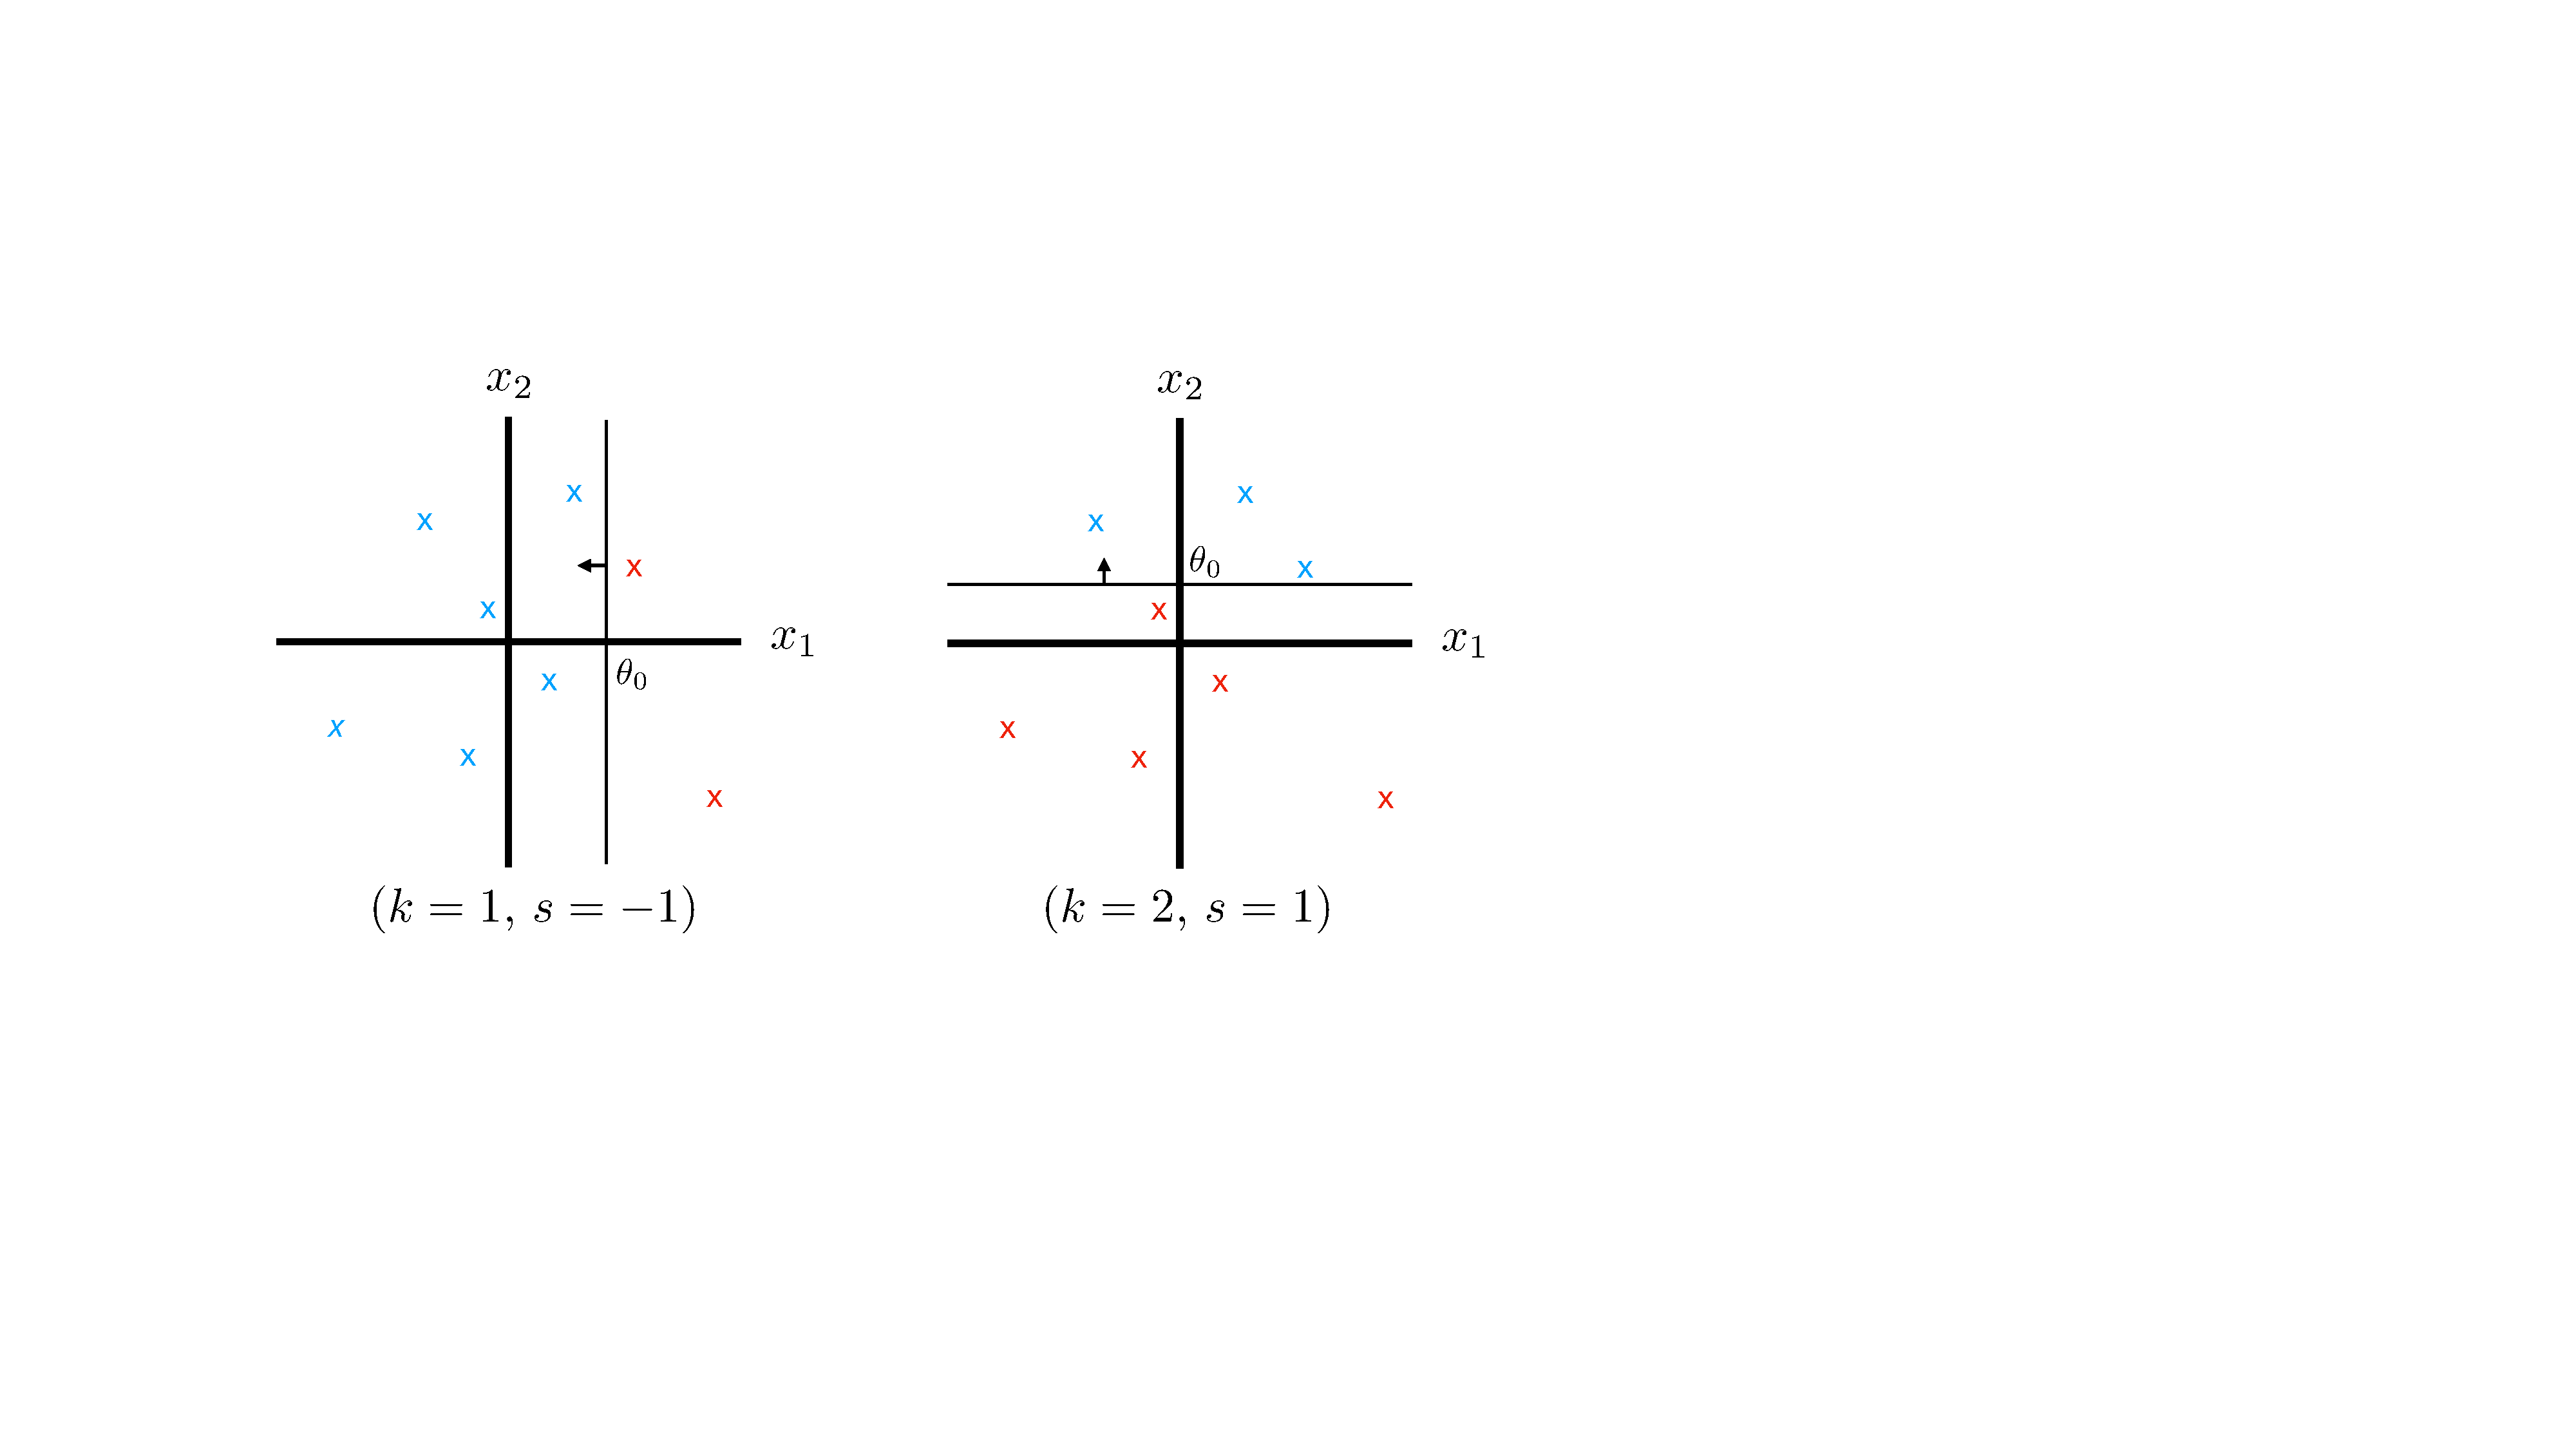
\includegraphics[width=.6\textwidth]{stump_example}
        \par
        \caption{Two examples of decision stumps, each applied to the same unlabeled data set.  The points classified as positive are colored blue, and the points classified as negative are colored red. \label{fig:stumps}}
    \end{figure}   

\subsection{The Algorithm}

AdaBoost takes as input the data set $\Dc$ and the number of iterations $M$, and performs the following steps:
\begin{enumerate}
    \item Initialize weights $w_0(t) = \frac{1}{n}$ for $t=1,\dotsc,n$.
    \item For $m=1,\dotsc,M$, do the following:
    \begin{enumerate}
        \item Choose the next base learner $h(\cdot;\hat{\btheta}_m)$ as follows:
        \begin{equation}
            \hat{\btheta}_m = \argmin_{\btheta}  \sum_{t \,:\, y_t \ne h(\xv_t;\btheta)} w_{m-1}(t). \label{eq:boost_theta}
        \end{equation}
        \item Set $\hat{\alpha}_m = \frac{1}{2} \log \frac{1 - \hat{\epsilon}_m}{\hat{\epsilon}_m}$, where $\hat{\epsilon}_m = \sum_{t \,:\, y_t \ne h(\xv_t;\hat{\btheta}_m)}^n w_{m-1}(t)$ is the minimal value attained in \eqref{eq:boost_theta}.
        \item Update the weights:
        \begin{equation}
            w_m(t) = \frac{1}{Z_m} w_{m-1}(t) e^{-y_t h(\xv_t;\hat{\btheta}_m) \hat{\alpha}_m } \label{eq:boost_w}
        \end{equation}
        for each $t=1,\dotsc,n$, where $Z_m$ is defined so that the weights sum to one:
        \begin{equation}
            Z_m = \sum_{t=1}^n w_{m-1}(t) e^{-y_t h(\xv_t;\hat{\btheta}_m) \hat{\alpha}_m }.  \label{eq:Zm}
        \end{equation}
    \end{enumerate}
    \item Output $f_M(\xv) = \sum_{m=1}^M \hat{\alpha}_m h(\xv; \hat{\btheta}_m)$, corresponding to the classifier $\hat{y}= \sign(f_M(\xv))$.
\end{enumerate}

We proceed by providing some intuition behind each of the main steps.  For step (a), we refer to
\begin{equation}
    \epsilon_m = \sum_{t \,:\, y_t \ne h(\xv_t;\btheta)} w_{m-1}(t)
\end{equation}
as {\em weighted training error}. The selection rule \eqref{eq:boost_theta} is choosing a base learner that ``classifies best'' when certain samples are treated as more important than others, as dictated by the weights $w_{m-1}(\cdot)$.

To understand the weight update rule \eqref{eq:boost_w} in step (c), it is useful to note that the quantity $-y_t h(\xv_t;\btheta)$ only takes values $+1$ or $-1$, and as a result, \eqref{eq:boost_w} can be rewritten as 
    \begin{equation}
        w_m(t) = \frac{1}{Z_m} w_{m-1}(t) \times
        \begin{cases}
            e^{\hat{\alpha}_m} & y_t \ne h(\xv_t;\hat{\btheta}_m) \\
            e^{-\hat{\alpha}_m} & y_t = h(\xv_t;\hat{\btheta}_m).
        \end{cases} \label{eq:update}
    \end{equation}
As a result, we are {\em increasing the weight} if the newly-chosen base learner classifies $\xv_t$ incorrectly, and {\em decreasing the weight} otherwise.  This aligns with the intuition given in Section \ref{sec:intro}; future iterations should place more importance on inputs that were previously classified wrongly. 

    \begin{figure}
        \centering
        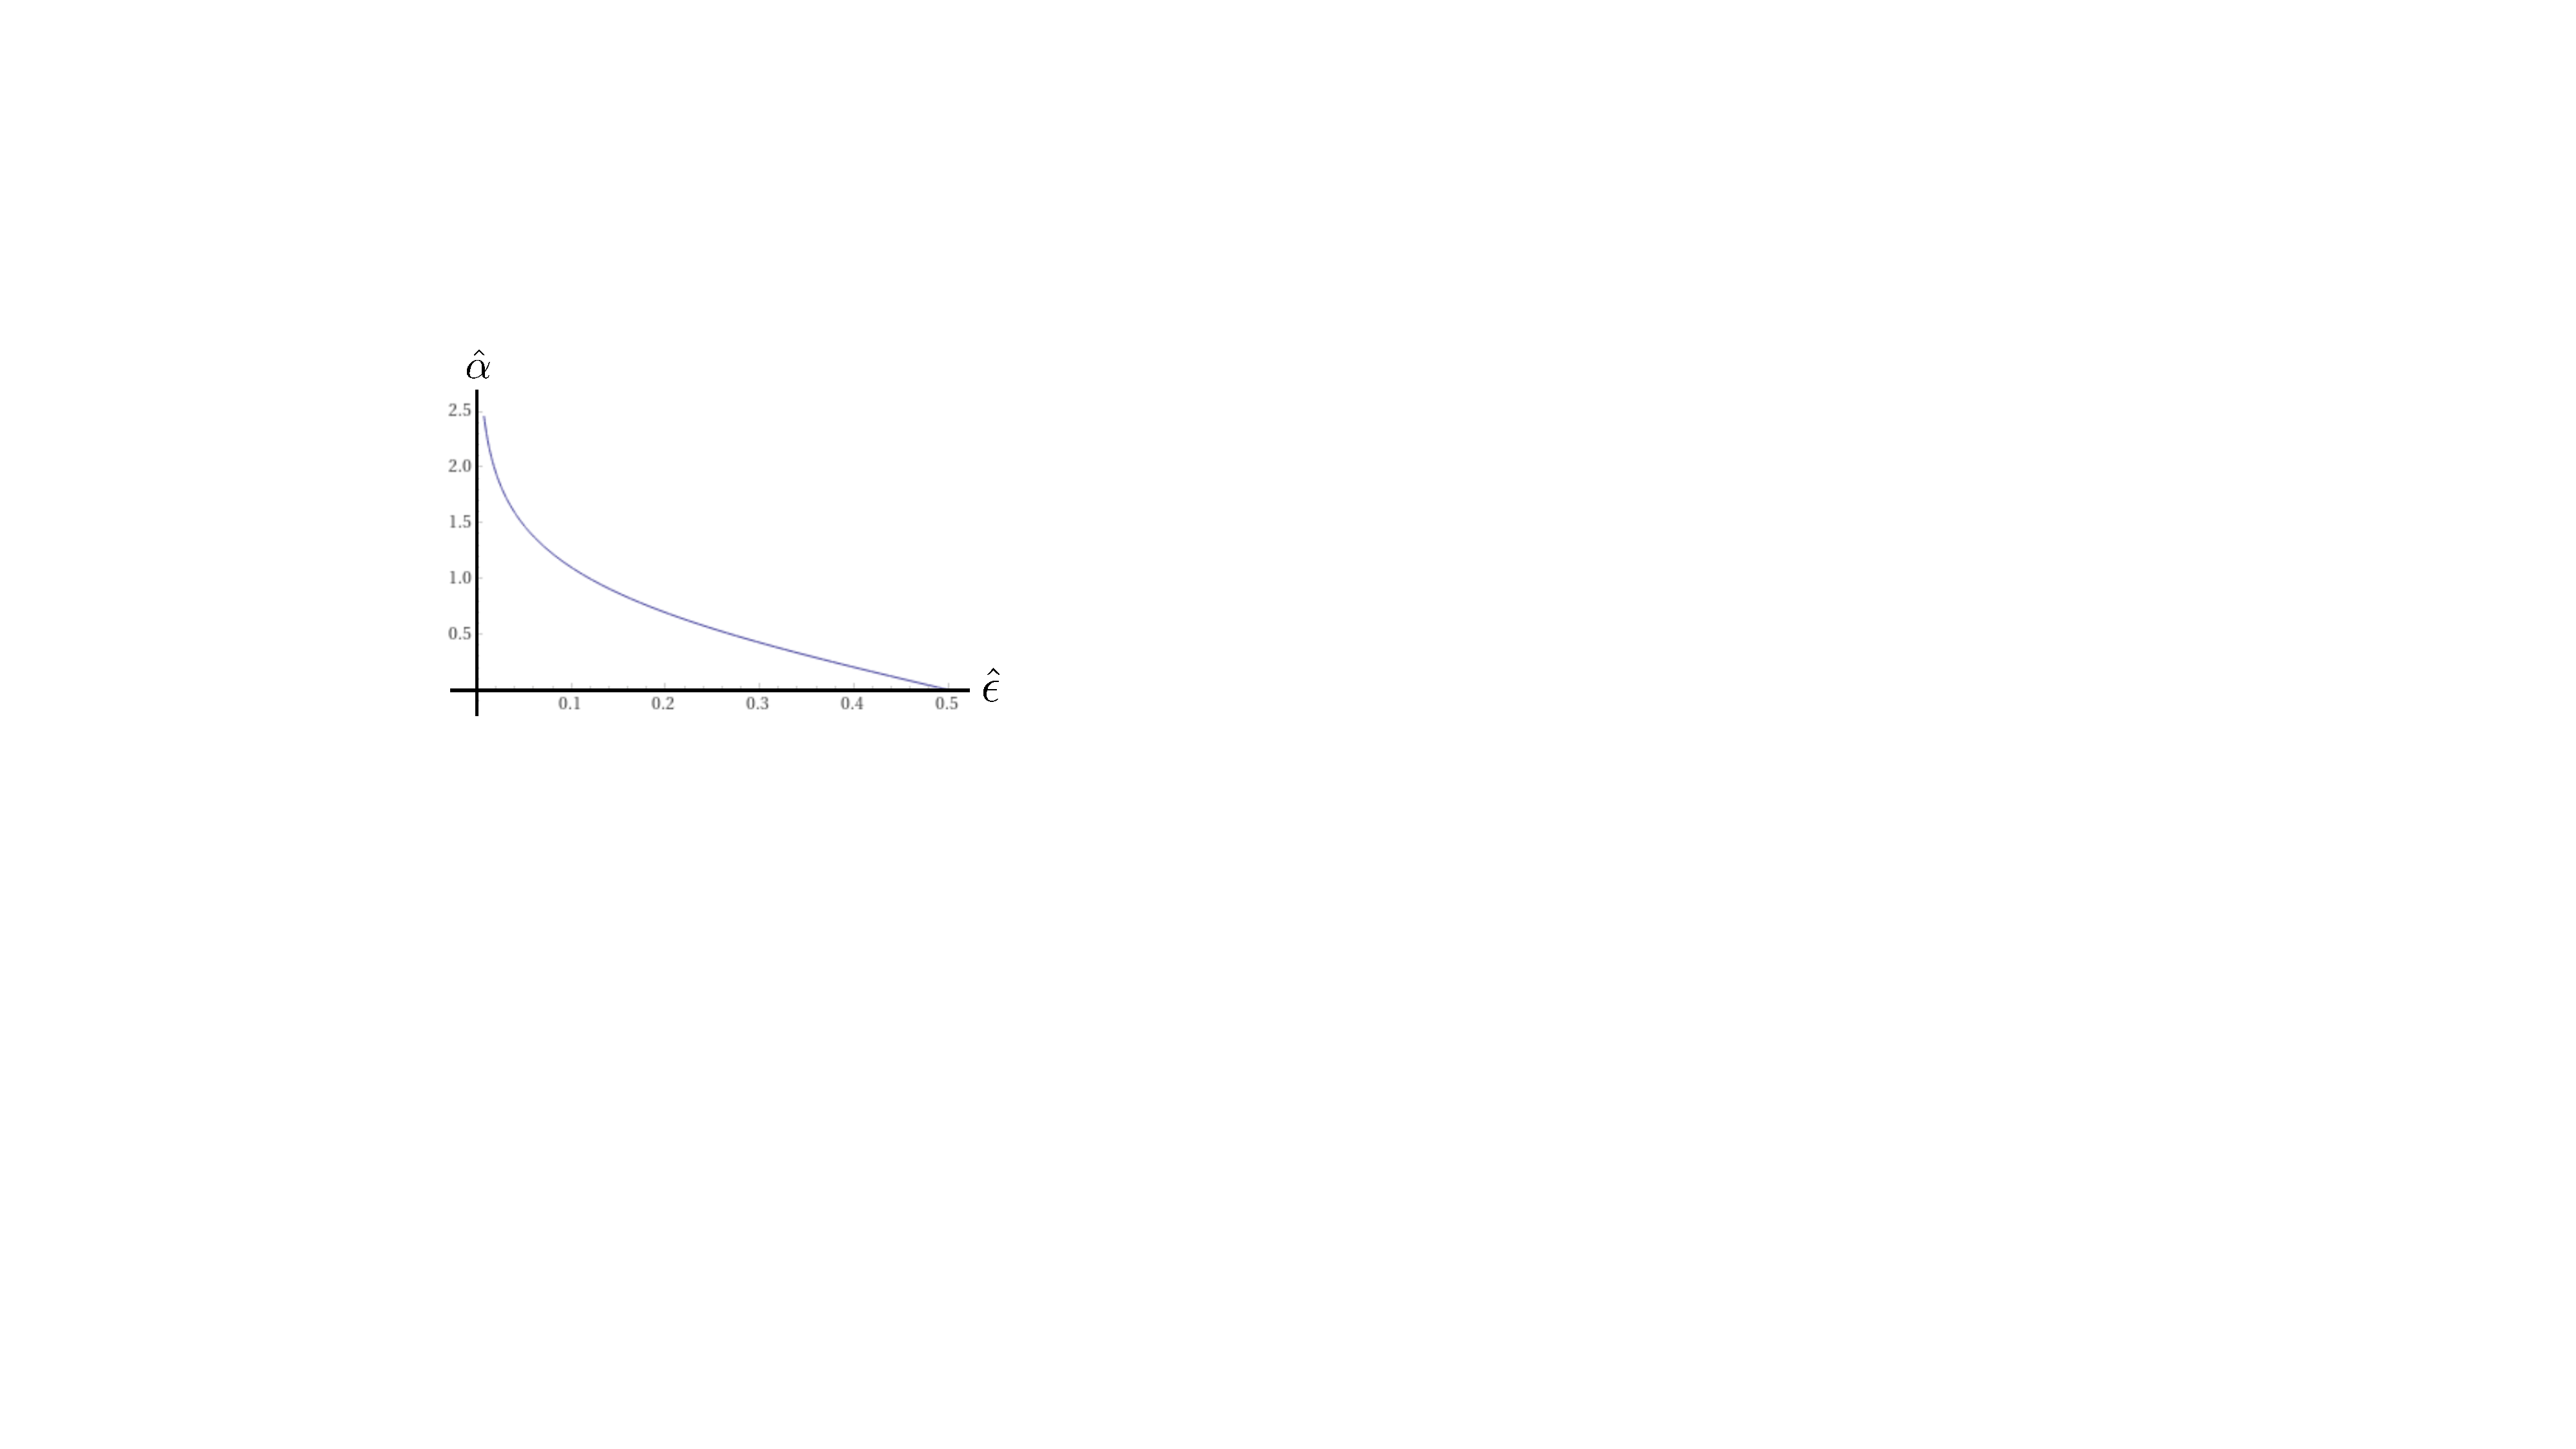
\includegraphics[width=.4\textwidth]{alpha_plot}
        \par
        \caption{Plot of $\hat{\alpha}_m$ as a function of $\hat{\epsilon}_m$. \label{fig:alpha_plot}}
    \end{figure}   

The choice of $\hat{\alpha}_m$ in step (b) arises from optimizing a certain expression in the mathematical analysis (see Section \ref{sec:math}), but we can still give some intuition behind it here.  In Figure \ref{fig:alpha_plot}, we plot this choice of $\hat{\alpha}_m$ as a function of $\hat{\epsilon}_m$, and observe that it is a decreasing function.  We therefore have the intuitive property that a higher vote is given to a base learner that has a lower weighted training error.  In the extreme cases, we have the following:
\begin{itemize}
    \item If $\hat{\epsilon}_m = 0$, then we have a ``perfect'' base learner, so it receives an infinitely large vote.  However, this case will only occur in a data set where a single decision stump can classify all points correctly, which is not to be expected.
    \item If $\hat{\epsilon}_m = \frac{1}{2}$, then we have a ``useless'' base learner, since even random guessing has a 50\% success rate.  Hence, in this case, the base learner receives a vote of zero.
\end{itemize}
We note that the case $\hat{\epsilon}_m > \frac{1}{2}$ will never be encountered in \eqref{eq:boost_theta}, because if we have a decision stump with weighted training error greater than $\frac{1}{2}$, then flipping its sign will make the weighted training error less than half.  Hence, the latter will be preferred by the minimization performed in \eqref{eq:boost_theta}.

\subsection{Experimental Examples}

In Figure \ref{fig:exp}, we show the results of running AdaBoost for $M=50$ iterations, using two different data sets with $n=400$ points.  The $\xv_t$ values were chosen uniformly at random from $[-1,1]^2$, and their labels were assigned according to the ``ground truth'' image shown.

We see that AdaBoost is able to roughly recover the shapes of the classification functions that were used to generate the data.  On the other hand, the ``blocky'' behavior of the final output could be considered undesirable.  This behavior arises from the use of the {\em extremely simple} decision stump class for the base learner; see Section \ref{sec:ext} for further discussion. 

    \begin{figure}
        \centering
        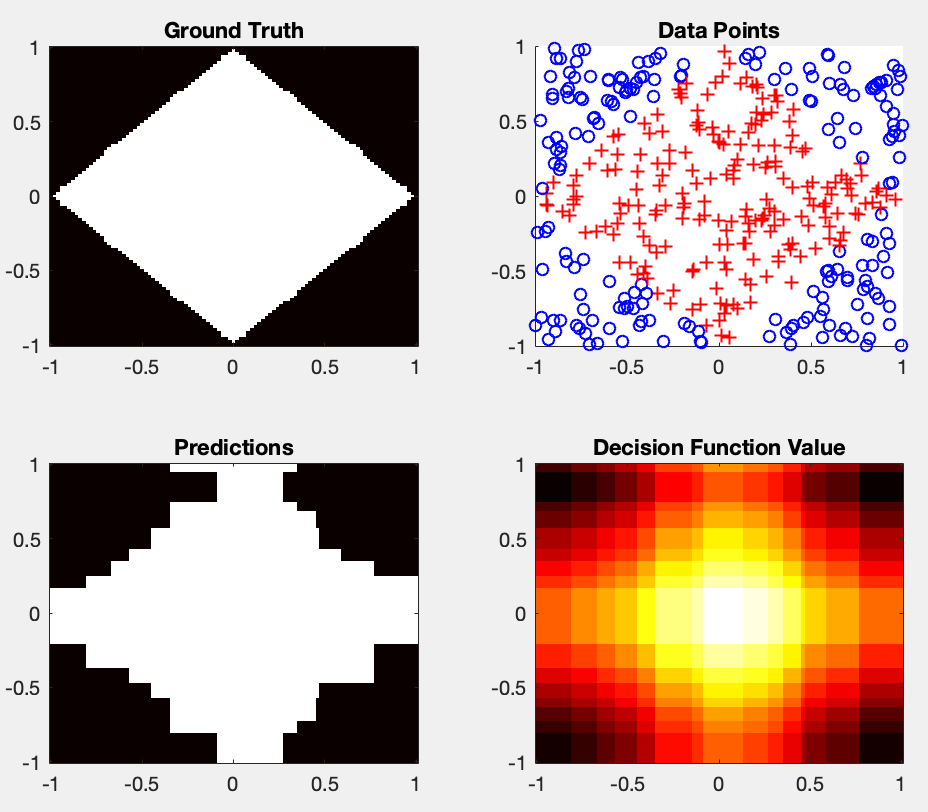
\includegraphics[width=.43\textwidth]{BoostingExp1} ~~~~~
        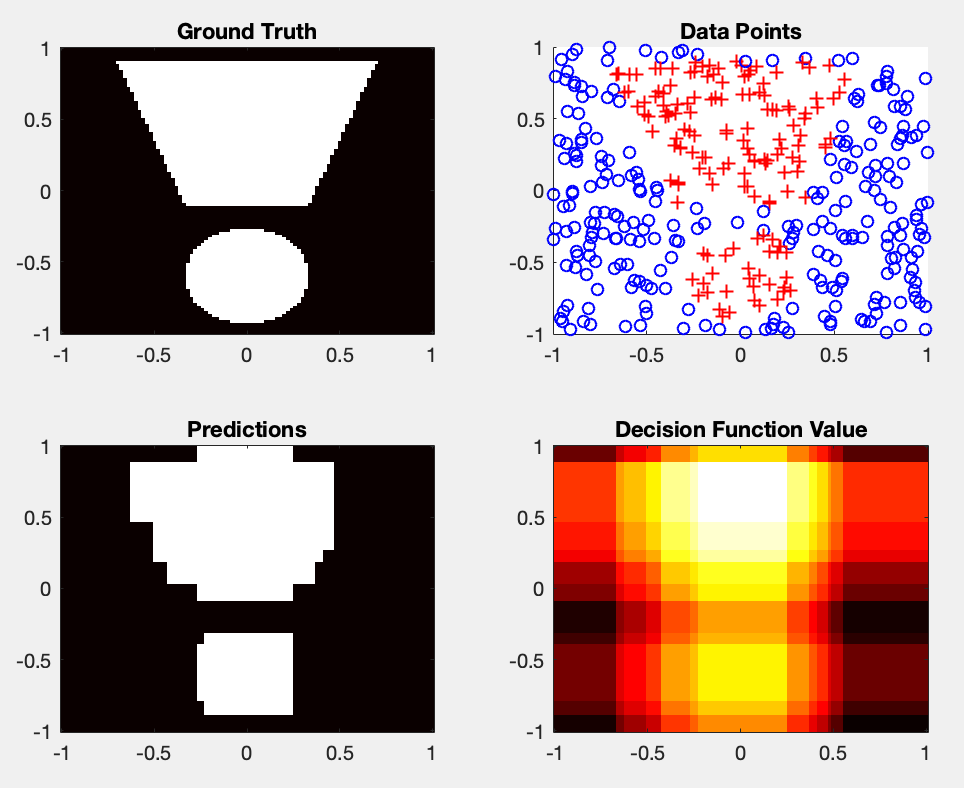
\includegraphics[width=.46\textwidth]{BoostingExp2}
        \par
        \caption{Experimental results for AdaBoost on two data sets with $n=400$ data points and $M=50$ boosting iterations.  The bottom-right of each example shows a color map of the function $f_M(\xv)$, and taking its sign gives the predictions shown in the bottom-left. \label{fig:exp}}
    \end{figure}  

\section{Mathematical Analysis} \label{sec:math}

An elegant theoretical result on the AdaBoost algorithm states that as long as each base learner performs {\em slightly better} than random guessing (i.e., slightly better weighted training error than $\frac{1}{2}$), the proportion of misclassified points in $\Dc$ is guaranteed to decrease {\em exponentially fast} in the number of iterations $M$.  This is formally stated in the following.

\begin{thm} \label{thm:main}
    For any data set $\Dc = \{(\xv_t,y_t)\}_{t=1}^n$, after $M$ iterations, the training error of AdaBoost satisfies
    \begin{equation}
        \frac{1}{n}\sum_{t=1}^n \openone\{ y_t \ne \sign(f_M(\xv_t)) \} \le \exp\bigg( -2\sum_{m=1}^M \Big(\frac{1}{2}-\hat{\epsilon}_m\Big)^2 \bigg). \label{eq:main_result}
    \end{equation}
    In particular, if $\hat{\epsilon}_m \le \frac{1}{2} - \gamma$ for all $m$ and some $\gamma > 0$, then
    \begin{equation}
        \frac{1}{n}\sum_{t=1}^n \openone\{ y_t \ne \sign(f_M(\xv_t)) \}  \le e^{-2M\gamma^2}. \label{eq:boosting2}
    \end{equation}
\end{thm}
This result makes no explicit assumptions on the data set (e.g., linear separability), but rather only assumes $\hat{\epsilon}_m \le \frac{1}{2} - \gamma$, i.e., slightly outperforming random guessing.  It is also interesting to note that since the left-hand side of \eqref{eq:boosting2} only takes values in $\big\{0,\frac{1}{n},\dotsc\big\}$, the training error is zero for $M > \frac{\log n}{2\gamma^2}$.

We only provide a brief outline of the proof of Theorem \ref{thm:main} here, and provide the details in the appendix:
\begin{itemize}
    \item The first step is to upper bound the weighted training-error in terms the  {\em exponential loss}, defined as
    \begin{equation}
        \Loss_{\rm exp}(y, f(\xv)) = \exp(- y f(\xv)). \label{eq:loss_exp}
    \end{equation}
    Also defining the usual $0$-$1$ loss $\Loss_{01}(y,f(\xv)) = \openone\{ y \ne \sign( f(\xv) ) \}$, a simple plot of the two losses can be used to establish that $\Loss_{01}(y,f(\xv)) \le \Loss_{\rm exp}(y, f(\xv))$, and hence the training error satisfies
    \begin{equation}    
        \frac{1}{n}\sum_{t=1}^n\openone\{ y_t \ne \sign(f_M(\xv_t)) \} \le \frac{1}{n}\sum_{t=1}^n e^{-y_t f_M(\xv_t)}. \label{eq:step1}
    \end{equation}
    \item The second step is to rewrite the right-hand side of \eqref{eq:step1} as follows:
    \begin{equation}
        \frac{1}{n}\sum_{t=1}^n e^{-y_t f_M(\xv_t)} = \prod_{m=1}^M Z_m. \label{eq:step2}
    \end{equation}  
    While this is an unusual identity, it follows by a fairly simple recursion argument in which we write $w_0(t) = \frac{1}{n}$, then use the weight update expression \eqref{eq:boost_w} to write $w_1(t)$ in terms of $Z_1$, $w_2(t)$ in terms of $Z_1$ and $Z_2$, and so on, up to $w_M(t)$ in terms of $Z_1,\dotsc,Z_M$.  The fact that $\sum_{t=1}^n w_M(t) = 1$ can then be used to establish \eqref{eq:step2}.
    \item The remaining steps use some algebraic manipulations to characterize each $Z_m$ and upper bound it in terms of simpler quantities.  First, the definition of $Z_m$ is simplified to $e^{\hat{\alpha}_m} \hat{\epsilon}_m + e^{-\hat{\alpha}_m}(1 - \hat{\epsilon}_m)$, and then solving $\frac{\partial Z_m}{\partial \hat{\alpha}_m} = 0$ shows that the choice $\hat{\alpha}_m = \frac{1}{2} \log \frac{1 - \hat{\epsilon}_m}{\hat{\epsilon}_m}$ gives the smallest value of $Z_m$, and that this value simplifies to
    \begin{equation}
        Z_m = \sqrt{ 1 - (1-2\hat{\epsilon}_m)^2 }. \label{eq:Z_expression}
    \end{equation}
    With some additional tedious but basic algebraic manipulations, \eqref{eq:Z_expression} can then be further upper bounded as follows:
    \begin{equation}
        Z_m \le \exp\Big( -\frac{1}{2} (1-2\hat{\epsilon}_m)^2 \Big). \label{eq:Z_expression2}
    \end{equation}
    Combining \eqref{eq:Z_expression2} with \eqref{eq:step1}--\eqref{eq:step2}, we obtain the desired result in \eqref{eq:main_result}.
\end{itemize}

\section{Extensions and Further Results} \label{sec:ext}

In this section, we briefly outline some more advanced algorithms and theory building on the previous sections.  Due to space limitations, we only provide a short discussion on each of these.

\subsection{Base Learners Beyond Decision Stumps} \label{sec:base}

In principle, any class of base learners could be used, instead of only decision stumps.  The choice of base learner class requires a suitable balance between various factors -- having a more complex base learner may lead to more powerful classifiers and fewer boosting iterations being required (i.e., smaller $M$), but may also make the crucial selection step in \eqref{eq:boost_theta} computationally challenging.  In addition, overly complicated base learners may lead to problems with overfitting.  In practice, a generalization of decision stumps known as {\em decision trees} often provides a good balance of these competing factors \cite{blog}.

\subsection{Multi-Class Boosting} \label{sec:multi}

While classification problems are commonly assumed to be binary, {\em multi-class} problems are also of considerable practical interest (e.g., number recognition would have 10 classes, and digit recognition would have at least 36).  Techniques for converting binary classifiers to multi-class classifiers (e.g., one vs.~rest and one vs.~one) often pose significant practical limitations, e.g., see \cite[Section 4.1.2]{bishop2006pattern}.  Fortunately, AdaBoost permits a natural direct extension to the multi-class setting, both in terms of the algorithm and its underlying theory \cite{saberian2011multiclass}.  In addition, although it is usually described in the context of classification, it can even be applied to regression problems \cite{scikit}, in which the label $y$ is continuous rather than finite-valued.

\subsection{Characterization of the Test Error} \label{sec:test_error}

In the discussion after Theorem \ref{thm:main}, we concluded that the training error of AdaBoost decreases to zero when $M$ is large enough.  In general, zero training error in machine learning is {\em not} considered a good thing, as it suggests that the classifier may be overly complex and subject to overfitting.  Surprisingly, however, AdaBoost has been shown to exhibit quite the opposite behavior in practice:  The test error (i.e., the performance on data that was not used in training) remains small even when the training error is zero, and can even {\em continue to decrease} when AdaBoost is run for additional iterations after reaching zero training error.

A partial explanation for this phenomenon was given by Schapire {\em et al.}~\cite{schapire1998boosting} using the notion of {\em margin}.  Recalling that the proof of Theorem \ref{thm:main} is based on upper bounding the 0-1 loss by the exponential loss, we find that a very small exponential loss not only guarantees a low 0-1 loss, but also guarantees a {\em large margin} (i.e., $f_M(\xv)$ is not only positive, but is far from zero).  By exploiting this property and some advanced connections between margin and generalization, theoretical guarantees can be provided not only for the training error, but also the test error \cite{schapire1998boosting}.

 
% \renewcommand{\newblock}{}
\newpage
\bibliographystyle{plain}
\bibliography{refs}

\newpage
{\huge \centering \bf Appendix \par}

\appendix

\section{Proof of Theorem \ref{thm:main} (AdaBoost Training Error Guarantee)}

The proof proceeds in several steps.

\medskip
{\noindent \bf Step 1 (Convert to exponential loss):} As stated following \eqref{eq:loss_exp}, the exponential loss upper bounds the $0$-$1$ loss, so
    \begin{equation}    
        \frac{1}{n}\sum_{t=1}^n\openone\{ y_t \ne \sign(f_M(\xv_t)) \} \le \frac{1}{n}\sum_{t=1}^n e^{-y_t f_M(\xv_t)}. \label{eq:step1a}
    \end{equation}

\medskip
{\noindent \bf Step 2 (An unusual equality):} In this step, we show that
    \begin{equation}
        \frac{1}{n}\sum_{t=1}^n e^{-y_t f_M(\xv_t)} = \prod_{m=1}^M Z_m. \label{eq:step2a}
    \end{equation}  
To see this, we write out the weight updates recursively according to the initialization $w_(t) = \frac{1}{n}$ and the update rule \eqref{eq:boost_w}:
    \begin{gather*}
        w_0(t) = \frac{1}{n} \\
        w_1(t) = \frac{1}{n} \frac{ \exp(-\hat{\alpha}_1 y_t h(\xv_t; \btheta_1 )) }{Z_1} \\
        w_2(t) = \frac{1}{n} \frac{ \exp(-\hat{\alpha}_1 y_t h(\xv_t; \btheta_1 )) }{Z_1} \frac{ \exp(-\hat{\alpha}_2 y_t h(\xv_t; \btheta_2 )) }{Z_2} \\
        \vdots \\
        w_M(t) = \frac{1}{n}  \frac{\exp\big( -\sum_{m=1}^M \hat{\alpha}_m y_t h(\xv_t;\btheta_m) \big)}{ \prod_{m=1}^M Z_m } = \frac{1}{n} \cdot \frac{\exp\big( -y_t f_M(\xv_t) \big)}{ \prod_{m=1}^M Z_m },
    \end{gather*}
    where in the last step we substituted \eqref{eq:fM}.
    The desired claim follows since $\sum_{t=1}^M w_M(t) = 1$ by construction (i.e., by the definition of the weights in the algorithm).

\medskip
{\noindent \bf Step 3 (Rewriting $Z_m$):} Recall the definition of $Z_m$ in \eqref{eq:Zm}.  We can split the sum over $t$ into two cases: If $y_t = h(\xv_t;\hat{\btheta}_m)$ then $y_t h(\xv_t;\hat{\btheta}_m) = 1$, whereas if $y_t \ne h(\xv_t;\hat{\btheta}_m)$ then $y_t h(\xv_t;\hat{\btheta}_m) = -1$.  Therefore, \eqref{eq:Zm} simplifies to
\begin{align}
    Z_m &= \sum_{t\,:\,y_t \ne h(\xv_t;\hat{\btheta}_m)} e^{\hat{\alpha}_m} w_{m-1}(t) + \sum_{t\,:\,y_t = h(\xv_t;\hat{\btheta}_m)} e^{-\hat{\alpha}_m} w_{m-1}(t) \nonumber \\
        &= e^{\hat{\alpha}_m} \hat{\epsilon}_m + e^{-\hat{\alpha}_m}(1 - \hat{\epsilon}_m), \label{eq:Z_new}
\end{align} 
where we have used the fact that $\sum_{t\,:\,y_t \ne h(\xv_t;\hat{\btheta}_m)} w_{m-1}(t) = \hat{\epsilon}_m$ by definition, and we similarly have $\sum_{t\,:\,y_t = h(\xv_t;\hat{\btheta}_m)} w_{m-1}(t) = 1 - \hat{\epsilon}_m$ since the weights sum to one by definition.

Note that $\frac{\partial Z_m}{\partial \hat{\alpha}_m} = \hat{\epsilon}_m e^{\hat{\alpha}_m} - e^{-\hat{\alpha}_m}(1-\hat{\epsilon}_m)$; setting this to zero and solving gives $\hat{\alpha}_m = \frac{1}{2} \log \frac{1 - \hat{\epsilon}_m}{\hat{\epsilon}_m}$. It is easy to check that it is a minimum, and not a maximum.

\medskip
{\noindent \bf Step 4 (Substitute $\hat{\alpha}_m$ and simplify):} Substituting the choice of $\hat{\alpha}_m$ into \eqref{eq:Z_new} gives
    \begin{align}
        Z_m &= \sqrt{\frac{1-\hat{\epsilon}_m}{\hat{\epsilon}_m}} \hat{\epsilon}_m + \sqrt{\frac{\hat{\epsilon}_m}{1-\hat{\epsilon}_m}}(1 - \hat{\epsilon}_m) \\
            &= 2\sqrt{ \hat{\epsilon}_m (1-\hat{\epsilon}_m) } \\
            &= \sqrt{ 1 - (1-2\hat{\epsilon}_m)^2 }, \label{eq:blah}
    \end{align}
    where the last step can be verified by expanding the square.  The last line allows us to use the convenient inequality $\sqrt{1-c^2} = \exp\big( \frac{1}{2}\log( 1 - c^2 ) \big) \le \exp\big( - \frac{1}{2} c^2 \big)$m where the last step uses $\log(1+a) \le a$.  The motivation behind doing this is that products of exponentials are convenient, because they simplify to $\exp\big(\sum\dotsc)$.

    Applying this upper bound in \eqref{eq:blah} gives $Z_m \le \exp\big( -\frac{1}{2} (1-2\hat{\epsilon}_m)^2 \big)$, and combining with \eqref{eq:step1a}--\eqref{eq:step2a} gives
    \begin{align*}
        \frac{1}{n}\sum_{t=1}^n\openone\{ y_t \ne \sign(f_M(\xv_t)) \} 
            &\le \prod_{m=1}^M Z_m \\
            &\le \prod_{m=1}^M \exp\bigg( -\frac{1}{2} (1-2\hat{\epsilon}_m)^2 \bigg) \\
            &= \exp\bigg( -2\sum_{m=1}^M \Big(\frac{1}{2}-\hat{\epsilon}_m\Big)^2 \bigg),
    \end{align*}
    which proves the desired result in \eqref{eq:main_result}.
\end{document}